\chapter{Singleton}
\section{Intento}

Utile per assicurarsi che una classe abbia solo un'istanza e fornisci un punto di accesso globale ad essa.

(nel progetto utile per l'interfaccia di accesso al db, cioè nel dbInstance, e nei DAO)


%---
\section{Struttura}

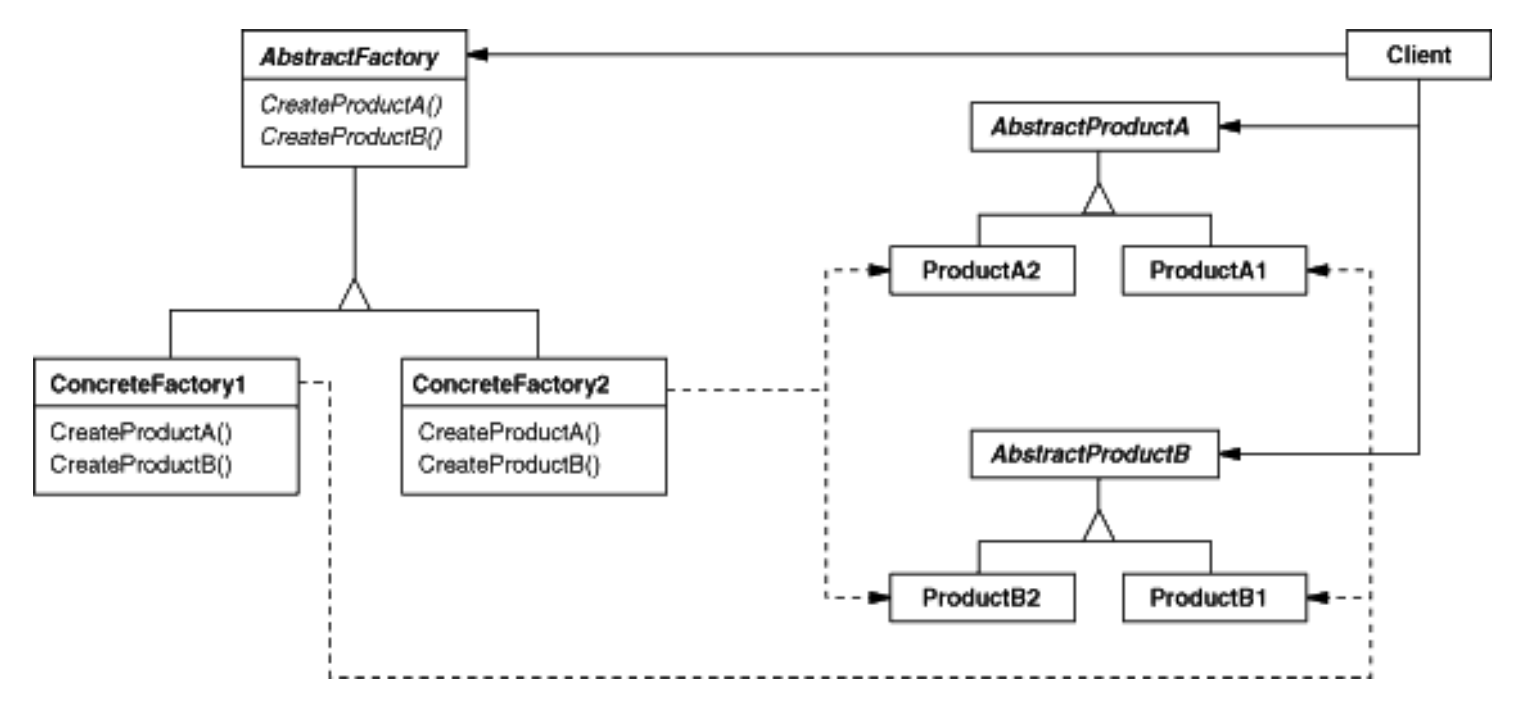
\includegraphics[width=\textwidth]{/Users/matt/Documents/GitHub/Design-Pattern-ITA/Singleton/Structure1}


%---
\section{Implementazione}

\subsection{Garantire un'istanza univoca.}
Il Singleton rende l'unica istanza un'istanza normale di una classe, ma quella classe è scritta in modo che possa essere creata solo un'istanza.

Un modo comune per eseguire questa operazione consiste nel nascondere l'operazione che crea l'istanza dietro una funzione statica, o un metodo di classe, che garantisce la creazione di una sola istanza. Questo approccio garantisce che un singleton venga creato e inizializzato prima del suo primo utilizzo.

È possibile definire l'operazione di classe con una funzione statica Istanza della classe Singleton. Singleton definisce anche una variabile statica "instance" che contiene un puntatore alla sua istanza univoca.
La classe Singleton è dichiarata come:

\begin{lstlisting}[language=java]
    public class SingleObject {
        private static SingleObject instance = new SingleObject();

        private SingleObject (){

        }

        public static SingleObject getInstance() {
            return instance;
        }
    }
\end{lstlisting}

I client accedono al Singleton esclusivamente tramite la funzione dell'istanza.

Notare che il costruttore è private. Un client che tenta di istanziare direttamente Singleton riceverà un errore in fase di compilazione. Ciò garantisce che solo un'istanza possa essere creata.

\subsection{Sottoclasse della classe Singleton.}
Il problema principale non è tanto definire la sottoclasse, ma installare la sua istanza univoca in modo che i client possano usarla. In sostanza, la variabile che fa riferimento all'istanza singleton deve essere inizializzata con un'istanza della sottoclasse. 

La tecnica più semplice consiste nel determinare quale Singleton si desidera utilizzare nell'operazione dell'istanza di Singleton. 

\begin{lstlisting}[language=java]
    MazeFactory Instance () {
        if (_instance == 0) {
            const char mazeStyle = getenv("MAZESTYLE");

            if (mazeStyle.equals("bombed")) {
                _instance = new BombedMazeFactory;
            } else if (mazeStyle.equals("enchanted")) {
                _instance = new EnchantedMazeFactory;
                // ... other possible subclasses
            } else {
                // default _instance = new MazeFactory;
            }

        }
        return _instance;
    }
\end{lstlisting}

Un altro modo per scegliere la sottoclasse di Singleton consiste nell'estrarre l'implementazione di Instance dalla classe genitore ed inserirla nella sottoclasse. Ciò consente di decidere la classe di Singleton al momento del collegamento ma la tiene nascosta ai client del singleton. Ma non è un approccio abbastanza flessibile.

Un approccio più flessibile utilizza un registro di Singleton. Invece di fare in modo che Instance definisca l'insieme di possibili classi Singleton, le classi Singleton possono registrare la loro istanza Singleton per nome in un registro noto.

Il registro esegue il mapping tra nomi di stringhe e Singleton. Quando l'istanza ha bisogno di un Singleton, consulta il registro, chiedendo il Singleton per nome. Il registro cerca il Singleton corrispondente, se esiste, e lo restituisce.

Questo approccio libera l'istanza dal conoscere tutte le possibili classi o istanze Singleton. Tutto ciò che richiede è un'interfaccia comune per tutte le classi Singleton che includa operazioni per il registro:

\begin{lstlisting}[language=java]
    class Singleton {
        static void Register(const char name, Singleton);
        static Singleton Instance();

        protected static Singleton Lookup(const char name);
        
        private static Singleton _instance;
        private static List<NameSingletonPair> _registry;
    }
\end{lstlisting}

Register registra l'istanza Singleton con il nome specificato. Per mantenere il registro semplice, faremo in modo che memorizzi un elenco di oggetti NameSingletonPair. Ogni NameSingletonPair associa un nome a un Singleton e l'operazione di ricerca trova un Singleton dato il suo nome.

\begin{lstlisting}[language=java]
    Singleton Instance () {
        if (_instance == 0) {
            const char singletonName = getenv("SINGLETON");
            // user or environment supplies this at startup
            
            _instance = Lookup(singletonName);
            // Lookup returns 0 if there's no such singleton
        }
        return _instance;
    }
\end{lstlisting}

Dove si registrano le classi Singleton? Una possibilità è nel loro costruttore. Ad esempio, una sottoclasse MySingleton potrebbe fare quanto segue:

\begin{lstlisting}[language=java]
    MySingleton() {
        // ...
        Register("MySingleton", this);
    }
\end{lstlisting}

Ovviamente, il costruttore non verrà chiamato a meno che qualcuno non istanzia la classe, il che fa eco al problema che il pattern Singleton sta cercando di risolvere! Possiamo aggirare questo problema definendo un'istanza statica di MySingleton:

\begin{lstlisting}[language=java]
    static MySingleton theSingleton;
\end{lstlisting}

La classe Singleton non è più responsabile della creazione del Singleton, infatti, la sua responsabilità primaria è rendere accessibile nel sistema l'oggetto di scelta Singleton.

L'approccio dell'oggetto statico ha ancora un potenziale svantaggio, ovvero che devono essere create istanze di tutte le possibili sottoclassi Singleton, altrimenti non verranno registrate.


%---
\section{Esempio Java}
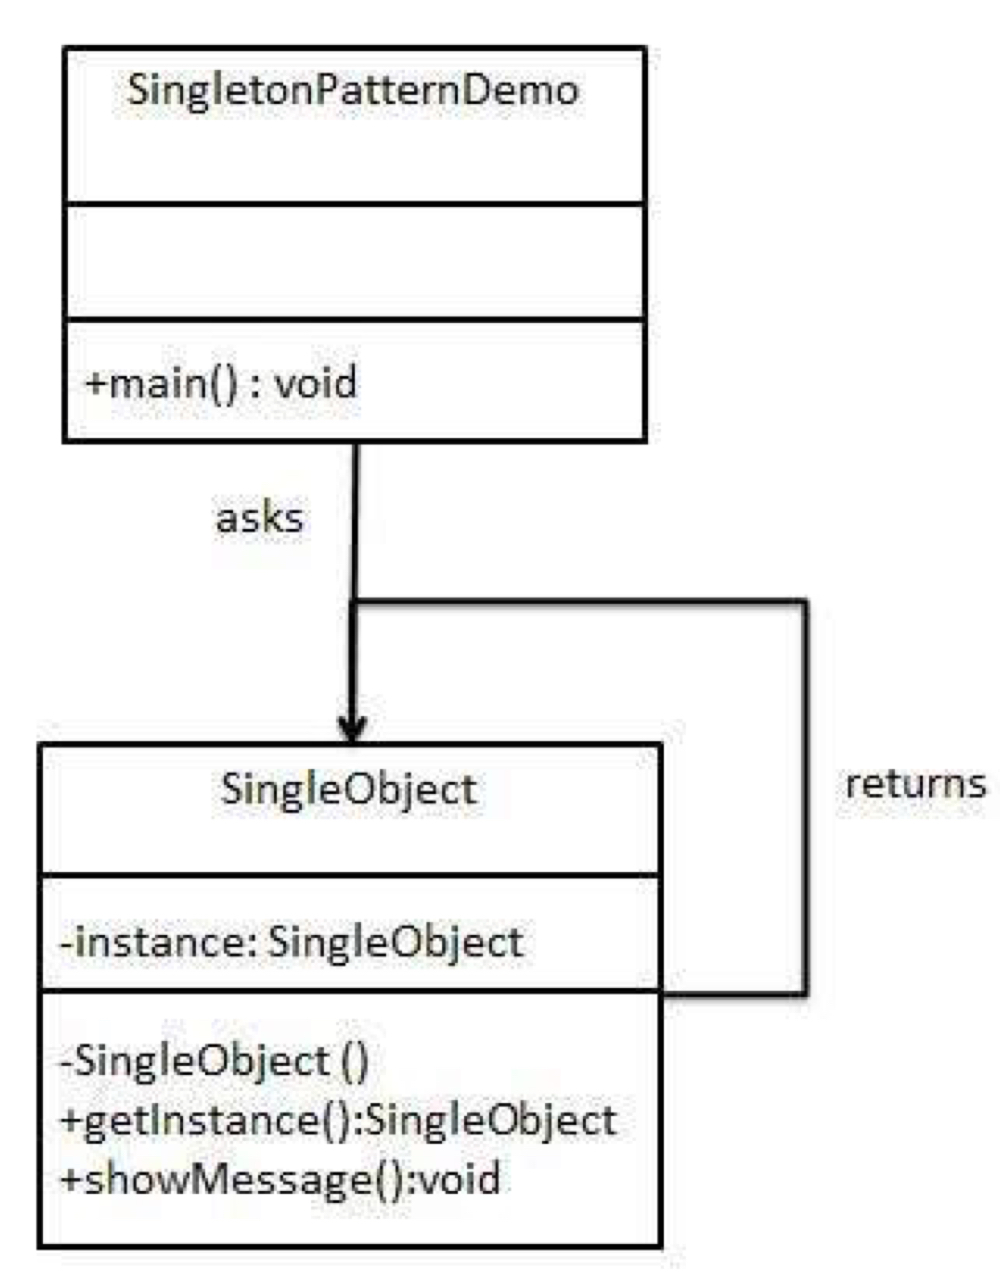
\includegraphics[width=7cm]{/Users/matt/Documents/GitHub/Design-Pattern-ITA/Singleton/Example1}

\subsection{Singleton.java}
\begin{lstlisting}[language=java]
    public class Singleton {
        private static Singleton instance = new Singleton();
    
        private Singleton (){
    
        }
    
        public static Singleton getInstance() {
             return instance;
        }
    
        public void showMessage(String message) {
            System.out.println(message);
        }
    }
\end{lstlisting}

\subsection{main}
\begin{lstlisting}[language=java]
    public static void main(String[] args) {
        Singleton so = Singleton.getInstance();

        so.showMessage("puppe");
    }
\end{lstlisting}